Totem jest prostym odtwarzaczem filmów. Dwukrotne kliknięcie na plik wideo w menadźerze plików spowoduje odtworznie go w programie Totem. Zaznaczenie wielu filmów w menadżerze plików i otworzenie ich w programie Totem dodaje je do kolejki odtwarzania. 

Totem korzysta z zainstalowanych w systemie kodeków. jeżeli zgodnie z tym przewodnikiem zainstalowałem pakiet \textcolor{ubuntu_orange}{ubuntu-restricted-extras} to Totem będzie wstanie odtworzyć każdy popularny format wideo.
\begin{center}
	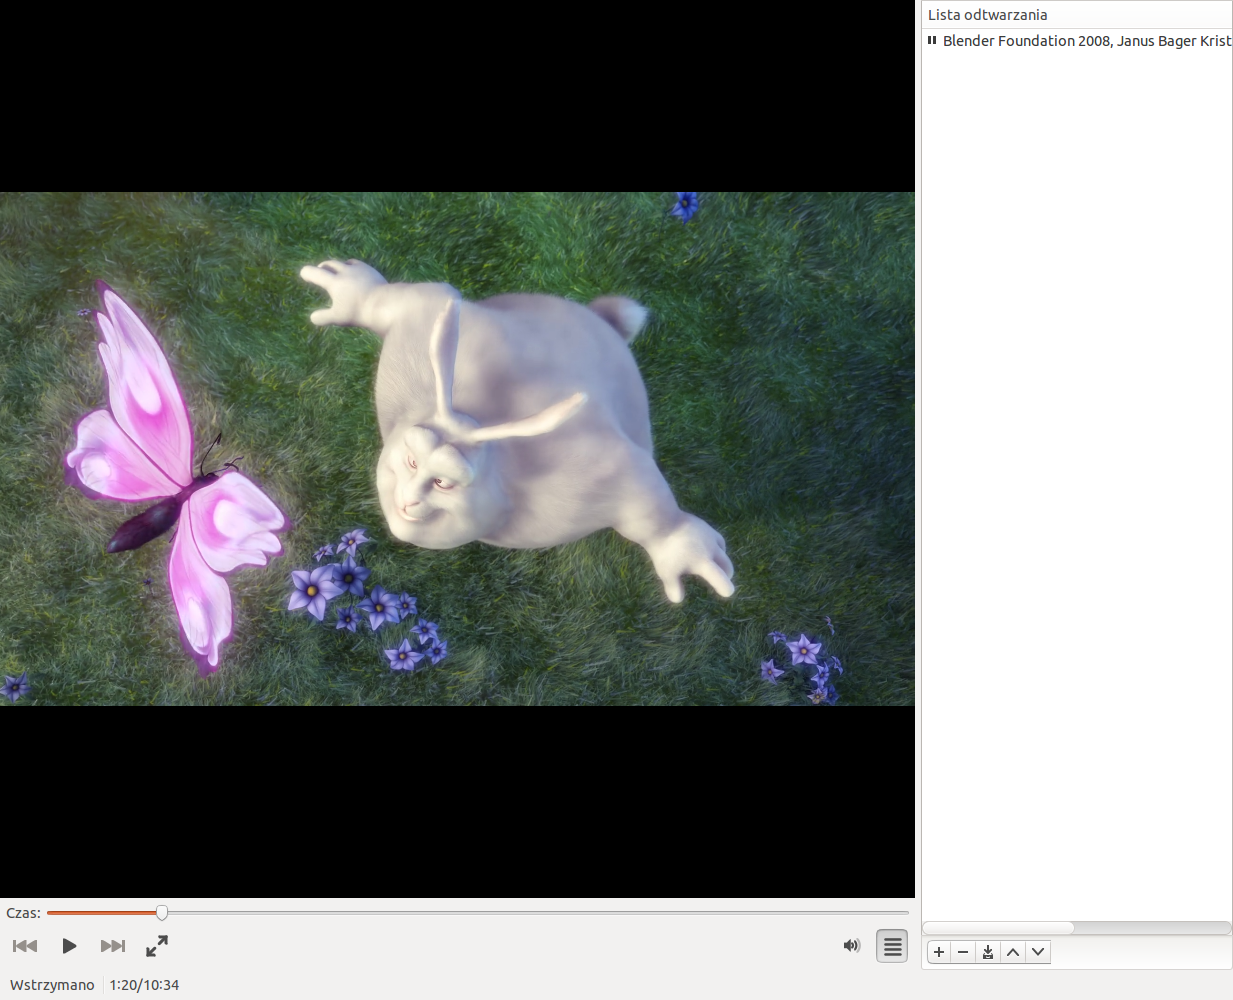
\includegraphics[width=\linewidth]{images/programy_totem1.png}
\end{center}

\subsubsection{Podstawy obsługi programu Totem}
Otwieranie plików:
\begin{itemize}
\item Wybierz \menu{{Film}>{Otwórz\ldots}} aby wskazać plik na lokalnym dysku.
\item Wybierz \menu{{Film}>{Otwórz z położenia\ldots}} aby wskazać plik w internecie, który ma zostac pobrany i odtworzony. Link do pliku musi być absolutny, tzn wskazywać bezpośrednio na film a nie na stronę z filmem.
\end{itemize}
Oglądanie filmu:
\begin{itemize}
\item Dwukrotne kliknięcie na obszarze oglądanego filmu uruchami tryb pełnoekranowy.
\item Klawisz \keys{\Space} wstrzymuje/wznawia odtwarzanie filmu.
\item Klawisz \keys{\arrowkeyright} przeskakuje jedną minutę do przodu.
\item Klawisz \keys{\arrowkeyleft} przeskakuje 15 sekund do tyłu.
\item Kółko myszy także pozwala na przemieszczanie się po filmie o ile kursor myszy znajduje się nad obszarem odtwarzania
\item Aby załadować napisamy wejdź w \menu{{Widok}>{Napisy}>{Wybierz plik z napisami}}
\end{itemize}